\documentclass[12pt, english]{article}
\usepackage{listings}
\usepackage{tikz}
\usepackage[most]{tcolorbox}
\usepackage[ampersand]{easylist}
\usetikzlibrary{calc}

% Introduction/Problem
% How to make splines
% How to use splines (Or any parametric for that matter) in a motion control fashion
% Building a suitable interface
% Problems faced when trying to get this to work
% Moditying splines on the fly, or using the robot's predicted position as a control point

% https://tex.stackexchange.com/questions/14967/source-code-listing-with-frame-around-code
\newtcblisting[auto counter]{code}[2][]{sharp corners, colframe=white, listing only, 
	listing options={basicstyle=\ttfamily,language=c++}, 
title=Listing \thetcbcounter: #2, #1}

\title{ Path planning from scratch }
\author{
	Team 955 (Duncan Freeman)
}

\begin{document}
\maketitle
\tableofcontents
\pagebreak

\section{The problem}
In FRC, we always have an autonomous period with an objective that requires us to move around. In many cases, the movement required is complex, must be generated on the fly (I.E. the field is different each time or the robot's position varies), and must have a precise result. There are a few ways to acheive this; Splines have the advantage of being easy to define, being fairly numerically stable, and relatively easy to generate. 
\par
Because we need such precise control, the Talon SRX (or it's derivatives) is a fine choice of motor controller, if not only for it's motion planning capabilities. Motion planning is essentially a method through which a PID loop can be controlled at a high sample rate (precision) using equiptment that may have high latency but adequate processing power. The Talon SRX usually receives commands for velocity or position control exactly at the moment they are required; When put in Motion Profile mode they allow the user to push a certain volume of closed loop commands and time intervals, and then they execute the result. Additionally, this buffer may be pushed to while the profile is in operation, allowing for extensive paths to be executed with extremely precise control. Usually, we just need profile outputs as velocities for left and right motors, as such:

\begin{table}[h!]
	\begin{center}
		\begin{tabular}{ | c | c | }
			\hline
			$t$ & $V_{\text{left}}$ \\
			\hline
			\hline
			0 & 2.3 \\
			1 & 2.1 \\
			2 & 2.9 \\
			3 & 3.4 \\
		\end{tabular}
		\quad
		\begin{tabular}{ | c | c | }
			\hline
			$t$ & $V_{\text{right}}$ \\
			\hline
			\hline
			0 & -1.9 \\
			1 & -2.1 \\
			2 & -2.9 \\
			3 & -1.9 \\
		\end{tabular}
		\caption{Motion profile example data}
	\end{center}
\end{table}

\par
In conclusion: We want motion profile data, and we're going to create it in real time using splines.

%Typical motion profile buffer:
%Two tables side by side, left and right motors with time in one column and vel in the other, cut off jagged at the bottom because there are more points

\pagebreak

\section{Going from A to B (splines)}
\subsection{Interpolation}
The basic element of path planning: We are at point $A$, we need to be at point $B$. Note that points $A$ and $B$ can be in any number of dimensions, but for the purpose of FRC this is mainly just 2 ($x$ and $y$). \\\par
The  simplest way to represent some sort of progression between $A$ and $B$ is through an \textit{interpolation}. For some $0 \leq k \leq 1$, an interpolation between an $A$ and $B$ of any number of dimensions is:
\[ D = A(1-k) + kB \]

\par
where $D$ is the point we are currently at. Note that $k$ doesn't have to represent time, and in the case of path planning most likely won't. 

\begin{center}
	\begin{tikzpicture}
		\node[outer sep=0pt,circle, fill,inner sep=1.5pt,label={[fill=white]left:$A$}] (A) at (-1,-1) {};
		\node[outer sep=0pt,circle, fill,inner sep=1.5pt, label={[fill=white]right:$B$}] (B) at (2,1) {};	
		\node[outer sep=0pt,circle, fill,inner sep=1.5pt, label={[fill=white]above:$D$}] (D) at ($(A)!0.25!(B)$) {};	
		\draw (A) -- (B);
	\end{tikzpicture}
	\[ k = 0.25 \]
\end{center}

\par
Now what if we needed to have multiple paths? What if we need to move in any other motion than a straight path? What if we needed to start at one direction and end in another? Well, some of this can solved using multiple interpolations.

\begin{center}
	\begin{tikzpicture}
		\node[outer sep=0pt,circle, fill,inner sep=1.5pt,label={[fill=white]left:$A$}] (A) at (-1,-1) {};
		\node[outer sep=0pt,circle, fill,inner sep=1.5pt, label={[fill=white]right:$B$}] (B) at (2,1) {};	
		\node[outer sep=0pt,circle, fill,inner sep=1.5pt, label={[fill=white]left:$C$}] (C) at (-2,1.5) {};	
		\node[outer sep=0pt,circle, fill,inner sep=1.5pt, label={[fill=white]above:$D$}] (D) at ($(B)!0.25!(C)$) {};	
		\draw (A) -- (B) -- (C);
	\end{tikzpicture}
	\[ k = 1.25,\,line=B \to C \]
\end{center}

\par
This \textit{does} work, and some teams do use it. You need to turn at point $B$, but that's not hard; It's just less flexible than splines.
\pagebreak

\subsection{Splines}
\par
Let's start with a simple spline with only 3 control points (The simplest spline has 2, and it's actually the interpolation you've already learned!):

\begin{center}
	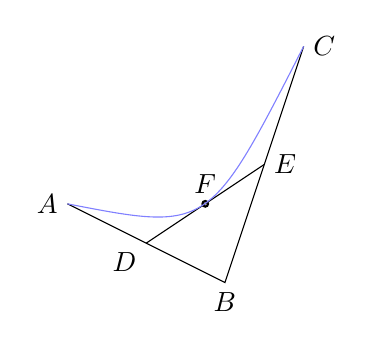
\begin{tikzpicture}
		\coordinate (A) at ( 0, 0);
		\coordinate (B) at ( 2,-1);
		\coordinate (C) at ( 3, 2);
		\draw (A) -- (B) -- (C);

		\coordinate (D) at ($(A)!0.5!(B)$);
		\coordinate (E) at ($(B)!0.5!(C)$);
		\draw (D) -- (E);

		\coordinate (F) at ($(D)!0.5!(E)$);

		\draw[thick] (F) circle(1pt) node[above] {$F$};
		\draw[color=blue!50] (A) .. controls (1.8, -0.35) .. (C);

		\node[left]  at (A) {$A$};
		\node[below] at (B) {$B$};
		\node[right] at (C) {$C$};
		\node[below left] at (D) {$D$};
		\node[right] at (E) {$E$};

	\end{tikzpicture}
\end{center}

\[ D = A(1-k) + kB \]
\[ E = B(1-k) + kC \]
\[ F = D(1-k) + kE \]

\[ k = 0.5 \]

In summary: \\
Go $k$ interval from $A$ to $B$ and call the point $D$. Go $k$ interval from $B$ to $C$ and call that point $E$. Do the same for $D$ and $E$ and call it $F$. As we increase $k$ from 0 to 1, $F$ moves along our spline (marked in blue). \\
\par
3 control points is fine for some cases, but we want to be able to connect two splines end-to-end to easily form a larger spline with $C_1$ continuity (Meaning that there are no sudden turns that have to be handled individually. We can write a cubic spline with 4 control points like so:
\begin{center}
	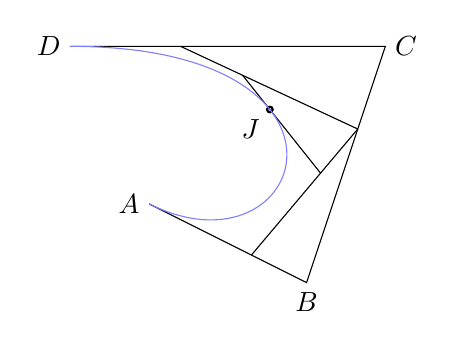
\begin{tikzpicture}
		\coordinate (A) at ( 0, 0);
		\coordinate (B) at ( 2,-1);
		\coordinate (C) at ( 3, 2);
		\coordinate (D) at (-1, 2);
		\draw (A) -- (B) -- (C) -- (D);

		\coordinate (E) at ($(A)!0.65!(B)$);
		\coordinate (F) at ($(B)!0.65!(C)$);
		\coordinate (G) at ($(C)!0.65!(D)$);
		\draw (E) -- (F);
		\draw (F) -- (G);

		\coordinate (H) at ($(E)!0.65!(F)$);
		\coordinate (I) at ($(F)!0.65!(G)$);
		\draw (H) -- (I);

		\coordinate (J) at ($(H)!0.65!(I)$);

		\node[left]  at (A) {$A$};
		\node[below] at (B) {$B$};
		\node[right] at (C) {$C$};
		\node[left]  at (D) {$D$};

		\draw[thick] (J) circle(1pt) node[below left] {$J$};
		\draw[color=blue!50] (A) .. controls (B) and (C) .. (D);

	\end{tikzpicture}
	\[ k = 0.65 \]
\end{center}

\[ E = A(1-k) + kB \]
\[ F = B(1-k) + kC \]
\[ G = C(1-k) + kD \]

\[ H = E(1-k) + kF \]
\[ I = F(1-k) + kG \]

\[ J = H(1-k) + kI \]

... phew! That was a lot. \\
\par

\subsection{Derivation}
If we write the whole expression out and simplify, it becomes this:
\[
	J=(1-k)^{3} A+3(1-k)^{2}k B+3(1-k)k^{2} C+k^{3}D
\]

It's somewhat uglier, but it's derivable. And when we do derive the expression, we get:
\[
   \frac{dJ}{dk}=3(1-k)^{2}(A-B)+6(1-k)k(C-B)+3k^{2}(D-C)
\]
... and the second derivative:
\[
	\frac{d^2J}{dk^2}=6(1-k)(C-2B+A)+6k( D-2C+B)
\]

Now that we know how to create the curve and it's derivatives, it's time to create the path(s).


\section{Path planning for \textit{any} parametric}

For this section, we will assume that the spline has been defined using 2 dimensional control points, and that $\frac{dx}{dk}$, $\frac{dy}{dk}$ are represented as $x'$ and $y'$.

\subsection{Wheel positions}
\begin{center}
	\scalebox{1.5}{%
		\begin{tikzpicture}
			\draw[step=1.0,gray,very thin] (-2.0,-2.0) grid (2.0,2.0);
			\draw (1.3, 0) -- (0, 1.3) -- (-1.3, 0) -- (0, -1.3) -- cycle;
			\node[circle,fill,inner sep=1pt] at (0,0) node[above right] {$J$};

			\coordinate (Right) at (-0.55,-0.55);
			\coordinate (Left) at (0.55,0.55);
			\draw (0,0) arc[radius = 3.7, start angle= 45, end angle= 80];
			\draw (0,0) arc[radius = 3.7, start angle= 45, end angle= 10];

			\draw (0,0) -- (Right) node[midway, above, sloped] {$w$};

			\draw[color=gray, dashed] (Right)  arc[radius = 3.0, start angle= 45, end angle= 75];
			\draw[color=gray, dashed] (Right)  arc[radius = 3.0, start angle= 45, end angle= 15];

			\draw[color=gray, dashed] (Left)  arc[radius = 4.5, start angle= 45, end angle= 82];
			\draw[color=gray, dashed] (Left)  arc[radius = 4.5, start angle= 45, end angle= 8];

			\draw[arrows=->] (-0.75,0.75) -- (0.75, -0.75);
		\end{tikzpicture}
	}
\end{center}

As shown in the diagram above, the spline defines where the \textit{center} of the robot will be. Our end goal is to find the rotational velocity of the individual wheels, so we need to figure out the position of each. $w$ represents the distance from the center of the robot to each of the wheel wells that define our physical robot.
\par
To find the position of a wheel at index $k$ along the spline, we need to find the perpendicular unit vector to our current motion $(x', y')$. Mulitplying it by $\pm w$ and adding it to position $J$ gives us the actual position of each wheel.

\[
	\begin{bmatrix}
		0 & -1 \\
		1 & 0 \\
	\end{bmatrix}
	\begin{bmatrix}
		x'(k)\\
		y'(k)\\
	\end{bmatrix}
	=
	\begin{bmatrix}
		-y'(k)\\
		x'(k)\\
	\end{bmatrix}
	= \{-y'(k), x'(k)\}
\]

\noindent
We then normalize the point by dividing it by the length of the original vector: \\
\[
	\label{deriv_speed_vec}
	\frac{\{-y'(k), x'(k)\}}{\sqrt{x'(k)^2+y'(k)^2}}
\]

\noindent
Adding the vector to the position along the curve gives us the final position of the wheel:
\[
	\{x(k), y(k)\} \pm d \left(\frac{\{-y'(k), x'(k)\}}{\sqrt{x'(k)^2+y'(k)^2}}\right)
\]

\noindent
Note: Either adding or subtracting  the vector to the position gives us two distict posibilities; These are the right and left wheels, respectively.

\subsection{Wheel velocities}
To find the velocity of each wheel, we can derive the position of each like so:
\[
	\{x'(k), y'(k)\} \pm d\frac{\{-y''(k), x''(k)\}*\sqrt{x'(k)^2+y'(k)^2} - \{-y'(k), x'(k)\} * \frac{y''(k)y'(k) + x''(k)x'(k)}{\sqrt{x'(k)^2+y'(k)^2}}}{x'(k)^2+y'(k)^2}
\]

\subsection{Reversing}
Because the rate of change in velocity must be positive for each motor, we have no intrinsic way of knowing if a given wheel should be in reverse to compensate for a tight corner. Luckily, there is a solution; we can find the rate of change in angle of center line, and measure if it's above/below $2\pi$. This works because if the rate of change is above $2\pi$ we're making a turn sharper than if one motor was at 100\% and the other at 0\%. We can find the derivate of the change in angle like so:
\[
	\label{change_in_angle}
	\frac{d}{dk} 
	\tan^{-1}{\left(\frac{y'(k)}{x'(k)}\right)} = 
	\frac{1}{1 + \left(\frac{y'(k)}{x'(k)}\right)^2} * \frac{y''(k)x'(k) - x''(k)y'(k)}{x'(k)^2}
\]


\subsection{Incrementing over spline indices}
To approximate how far along the spline we should move (in index units $k$) to reach our next time point, we first need to find the distance we predict we will travel for $j$ units of change; this can be acquired with the lengths of the velocity vectors for both wheels, selecting the largest one to make sure that no wheel goes faster than the max velocity. This gives us $\frac{dr}{dk}$. We specify what $\frac{dr}{dt}$ is in code, manually, as well as dt. \\
\\
\noindent
Where r = position, t = time, and j is an index in the spline:

\noindent
\begin{math}
	\frac{dr}{dk} = 
	\text{Largest velocity of the two sides over } dk\\
	\\
	\frac{dr}{dt} = \text{Maximum velocity we allow} \\
	\\
	\left(\frac{dr}{dk}\right)^{-1} * \frac{dr}{dt} = \frac{dk}{dt} \\
	\\
	\frac{dk}{dt} * dt = dk \text{ required}
\end{math}

\end{document}
